


\newsavebox{\detectextrema}
\begin{lrbox}{\detectextrema} 
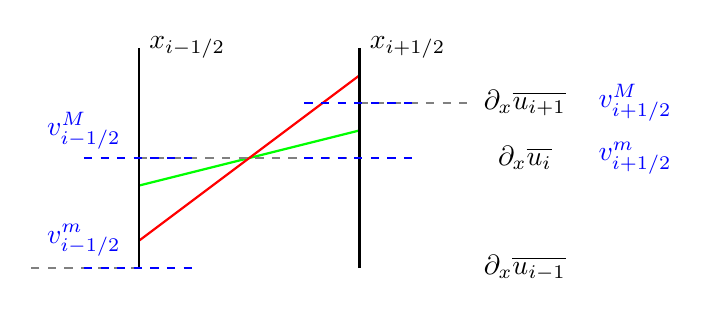
\begin{tikzpicture}[scale=0.7]
\draw[green, thick] (-2,-1/2) -- (2,1/2);
\draw[red,   thick] (-2,-3/2) -- (2,3/2);
\draw[black, thick] (-2,-4/2) -- (-2,4/2) node[right] {$x_{i-1/2}$};
\draw[black, thick] ( 2,-4/2) -- ( 2,4/2) node[right] {$x_{i+1/2}$};
\draw[gray,  thick,dashed] (-2, 0/2) -- (2,0/2);
\draw[gray,  thick,dashed] (-2, -4/2) -- (-4,-4/2);
\draw[gray,  thick,dashed] (2, 2/2)  -- ( 4,2/2);

\draw[blue,  thick,dashed] (-3,-4/2)  -- (-1,-4/2);
\draw[blue,  thick,dashed] (-3, 0/2)  -- (-1, 0/2);

\draw[blue,  thick,dashed] (1, 0/2)  -- ( 3,0/2);
\draw[blue,  thick,dashed] (1, 2/2)  -- ( 3,2/2);

\coordinate (s1) at (5,0) ;\coordinate (s2) at (5,1) ;\coordinate (s3) at (5,-2);
\coordinate (s4) at (7,0) ;\coordinate (s5) at (7,1) ;
\coordinate (s6) at (-3,0.5) ;\coordinate (s7) at (-3,-1.5) ;
\node at (s1) {$\partial_x \overline{u_i}$};
\node at (s2) {$\partial_x \overline{u_{i+1}}$};
\node at (s3) {$\partial_x \overline{u_{i-1}}$};

\node[blue] at (s4) {$v_{i+1/2}^m$};\node[blue] at (s5) {$v_{i+1/2}^M$};
\node[blue] at (s7) {$v_{i-1/2}^m$};\node[blue] at (s6) {$v_{i-1/2}^M$};
\end{tikzpicture}
\end{lrbox} 




\newsavebox{\Riemann}
\begin{lrbox}{\Riemann} 
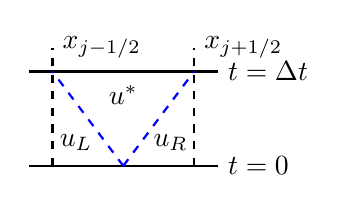
\begin{tikzpicture}[scale=0.6]

\draw[black, thick] (-2,0) -- (2,0) node[right] {$t=0$};
\draw[black, thick] (-2,2) -- (2,2) node[right] {$t=\Delta t$};
\draw[blue, thick,dashed](0,0) -- (1.5,2);
\draw[blue, thick,dashed](0,0) -- (-1.5,2);
\draw[black, thick,dashed](1.5,0) -- (1.5,2.5)  node[right]{$x_{j+1/2}$};
\draw[black, thick,dashed](-1.5,0) -- (-1.5,2.5)node[right]{$x_{j-1/2}$};


\coordinate (s1) at (0,1.5) ;\coordinate (s2) at (-1.,0.5) ;\coordinate (s3) at (1,0.5);

\node at (s1) {$u^*$};
\node at (s2) {$u_L$};
\node at (s3) {$u_R$};

\end{tikzpicture}
\end{lrbox} 


\newsavebox{\smaillage}
\begin{lrbox}{\smaillage} 
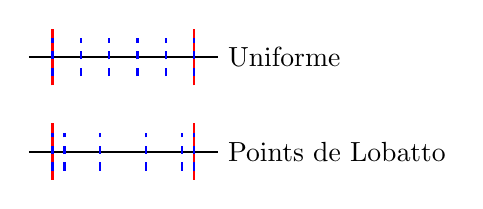
\begin{tikzpicture}[scale=0.6]

\draw[black, thick] (-2,0) -- (2,0) node[right] {Points de Lobatto};
\draw[black, thick] (-2,2) -- (2,2) node[right] {Uniforme};

\draw[red, thick] (-1.5,-0.6) -- (-1.5, 0.6);
\draw[red, thick] ( 1.5,-0.6) -- ( 1.5, 0.6);
\draw[blue, thick,dashed] (-1.5,-0.4) -- (-1.5, 0.4);
\draw[blue, thick,dashed] (-1.244,-0.4) -- (-1.244, 0.4);
\draw[blue, thick,dashed] (-0.4881,-0.4) -- (-0.4881, 0.4);
\draw[blue, thick,dashed] ( 0.4881,-0.4) -- ( 0.4881, 0.4);
\draw[blue, thick,dashed] ( 1.244,-0.4) -- ( 1.244, 0.4);
\draw[blue, thick,dashed] ( 1.5,-0.4) -- ( 1.5, 0.4);

\draw[red, thick] (-1.5, 1.4) -- (-1.5, 2.6);
\draw[red, thick] ( 1.5, 1.4) -- ( 1.5, 2.6);
\draw[blue, thick,dashed] (-1.5,1.6) -- (-1.5, 2.4);
\draw[blue, thick,dashed] (-0.9,1.6) -- (-0.9, 2.4);
\draw[blue, thick,dashed] (-0.3,1.6) -- (-0.3, 2.4);
\draw[blue, thick,dashed] ( 0.3,1.6) -- ( 0.3, 2.4);
\draw[blue, thick,dashed] ( 0.9,1.6) -- ( 0.9, 2.4);
\draw[blue, thick,dashed] ( 1.5,1.6) -- ( 1.5, 2.4);



\end{tikzpicture}
\end{lrbox} 


\newsavebox{\SRiemann}
\begin{lrbox}{\SRiemann} 
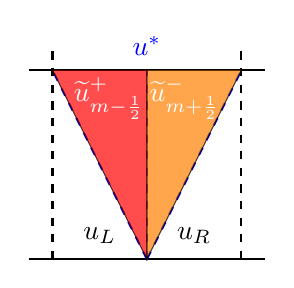
\begin{tikzpicture}[scale=0.6]

\draw[black, thick] (-2.5,-2) -- (2.5,-2);
\draw[black, thick] (-2.5,2) -- (2.5,2);
\draw[blue, thick,dashed](0,-2) -- (2.,2);
\draw[blue, thick,dashed](0,-2) -- (-2.,2);
\draw[black, thick,dashed](2.,-2) -- (2.,2.5)  ;
\draw[black, thick,dashed](-2.,-2) -- (-2.,2.5);

\draw[blue, thick,dashed](0,-2) -- (0,2);

\draw[fill=orange,opacity=0.7] (0,-2) -- (0,2) -- (2.,2) -- cycle;
\draw[fill=red,  opacity=0.7] (0,-2) -- (0,2) -- (-2.,2) -- cycle;

\coordinate (s1) at (0,2.5) ;\coordinate (s2) at (-1.,-1.5) ;\coordinate (s3) at (1,-1.5);
\coordinate (s4) at (-.8,1.4) ;\coordinate (s5) at (.8,1.4);
\node [text=blue]  at (s1) {$u^*$};
\node at (s2) {$u_L$};  \node [thick,text=white] at (s4) {$\widetilde{{u}}_{m-\frac{1}{2}}^+$};
\node at (s3) {$u_R$};  \node [thick,text=white] at (s5) {$\widetilde{{u}}_{m+\frac{1}{2}}^-$} ;

\end{tikzpicture}
\end{lrbox} 
